\section{Stregsensor}
På kørebanen til konkurrencen er der en hvis streg, som makere start. Det ønskes at kunne detektere dennne streg, for af vide hvornår bilen har kørt en omgang.\\
Til at dektektere start linjen, som er hvid skal den valgte sensor detekterer foreskellen mellem hvid og stort på banen.\\
 \\
Til det pågældende formål er en reflektiv optisk sensor blevet undersøgt og valgt. Den reflektive optiske sensore har fordelen at den er lille og fylder lidt.\\
\\

\subsection{CNY70}
\begin{wrapfigure}{r}{0.5\textwidth}
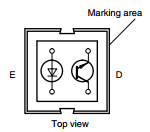
\includegraphics[scale=1.0]{./Graphics/CNY70-Diode}
\caption{billed af dioden og transisteren i CNY70}
\label{CNY70}
\end{wrapfigure}
Den refleksive optiske sensor som er valgt, hedder CNY70. Sensoren fylder $7x7x6$ mm og er placeret $0.2$ mm fra den overflade den operere på. \\
CNY70'eren er fastmonteret på undervognene af bilen, som vender ned mod banen.\\
\\
sensoren består af en diode og en fototransistor, da både diode og fototransistor vender ned mod banen, fungere den ved at lyset fra dioden reflektere i banen og fototransistoren opfangere det reflekterede lys og åbner alt efter hvor meget der bliver reflekteret. \\
\begin{wrapfigure}{r}{0.5\textwidth}
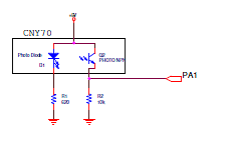
\includegraphics[scale=1.0]{./Graphics/Stregsensor_kredslob}
\caption{Det elektroniske kredsløb over stregsensoren}
\label{Stregsensor}
\end{wrapfigure}
Mørke farver absobere meget af lyset mens lyse farver reflektere dem. \\
(henvis til kredsløb for stregsensor)sensoren er forsynet med 5V, men kun når diodens stråler reflekteres åbner transistoren og udgangsspændingen på output-benet bliver højt.\\
Programmet til stregsensoren tjekker først på rising edge og registrere dette, så tjekker den for falling edge og registrere dette, microcontrolleren har nu dektekteret hele målstregen. \\

